\documentclass[12pt]{extarticle}
\usepackage{tempora}
\usepackage[T1, T2A]{fontenc}
\usepackage[utf8]{inputenc}
\usepackage[english, ukrainian]{babel}
\usepackage{geometry}
\usepackage{graphicx}
\usepackage{multirow}
\usepackage{multicol}
\usepackage{float}
\graphicspath{{/home/artem/Pictures}}
\geometry
{
    a4paper,
    left=30mm,
    top=15mm,
    right=20mm,
    bottom=15mm,
}

\begin{document}
\begin{titlepage}
    \begin{center}
        \textbf{\normalsize{\MakeUppercase{
            Міністерство Освіти і науки України
            Національний університет "Львівська політехніка"
        }}}

        \begin{flushright}
        \textbf{ІКНІ}\\
        Кафедра \textbf{ПЗ}
        \end{flushright}
        \vspace{15mm}

        \includegraphics[width=0.4\textwidth]{lpnu_logo.png}

        \vspace*{\fill}

        \textbf{\normalsize{\MakeUppercase{Звіт}}}
            
        До лабораторної роботи №1

        \textbf{на тему:} “ Метод сортування вибором.”

        \textbf{з дисципліни:} “Операційні системи”
            
        \vspace*{\fill}

        \begin{flushright}

            \textbf{Лектор:}\\
            доцент кафедри ПЗ\\
            Коротєєва Т.О.\\
            \vspace{12pt}

            \textbf{Виконав:}\\
            студент групи ПЗ-24\\
            Губик А. С.\\
            \vspace{12pt}

            \textbf{Прийняв:}\\
            асистент кафедри ПЗ\\
            Вишневський О. К.\\
        \vspace{12pt}
        \end{flushright}

        Львів -- 2023
            
            
    \end{center}
\end{titlepage}

\subsection*{Тема роботи} 
Метод сортування вибором.

\subsection*{Мета роботи} Вивчити алгоритм сортування вибором. 
Здійснити програмну реалізацію алгоритму сортування вибором.
 Дослідити швидкодію алгоритму сортування вибором.

\subsection*{Індивідуальне завдання}
Задано одномірний масив дійсних чисел. До парних елементів масиву застосувати функцію \space $\sqrt[]{|x -10|}$. Отриманий масив посортувати в порядку зростання.

\subsection*{Теоретичні відомості}
Сортування вибором (англійською «Selection Sort») — простий алгоритм сортування лінійного масиву, на основі вставок. Має ефективність O(n2), що робить його неефективним при сортування великих масивів, і в цілому, менш ефективним за подібний алгоритм сортування включенням. Сортування вибором вирізняється більшою простотою, ніж cортування включенням, і в деяких випадках вищою продуктивністю.

Алгоритм працює наступним чином:

1.     Знаходить у списку найменше значення.

2.     Міняє його місцями із першим значеннями у списку.

3.     Повторює два попередніх кроки, доки список не завершиться (починаючи з другої позиції).

Фактично, таким чином ми поділили список на дві частини: перша (ліва) — повністю відсортована, а друга (права) — ні.

Сортування вибором не є складним в аналізі та порівнянні його з іншими алгоритмами,
 оскільки жоден з циклів не залежить від даних у списку. 
 Знаходження найменшого елементу вимагає перегляду усіх n 
елементів (у даному випадку $(n - 1)$ порівняння), і після цього, 
перестановки його до першої позиції. Знаходження наступного найменшого 
елементу вимагає перегляду $(n - 1)$ елементів, і так далі, для 
$(n - 1) + (n - 2) + ... + 2 + 1 = n(n - 1) / 2 \theta(n^2)$ порівнянь. Кожне сканування 
вимагає однієї перестановки для $(n - 1)$ елементів (останній елемент знаходитиметься на своєму місці).

\subsection*{Покроковий опис}

\begin{enumerate}

\item \textbf{Ініціалізація:} Алгоритм починається з усього списку, 
який розглядається як невідсортована частина.

\item \textbf{Функція:} До парних елементів масиву застосовуємо $\sqrt[]{|x -10|}$.

\item \textbf{Пошук мінімуму:} Алгоритм шукає мінімальний елемент у 
невідсортованій частині списку. Це відбувається за допомогою
 порівняння кожного елемента в невідсортованій частині з поточним
  мінімумом.

\item \textbf{Обмін:} Після знаходження мінімального елемента він обмінюється з 
ліворуч найбільшим (або праворуч найменшим) елементом в
 невідсортованій частині. Це ефективно переміщує мінімальний елемент
  на початок відсортованої частини.

\item \textbf{Зменшення невідсортованої частини:} Відсортована частина 
тепер має на один елемент більше, а невідсортована на один елемент менше.
 Алгоритм повторює кроки 2 і 3 для залишкової невідсортованої частини,
  шукаючи мінімум серед залишкових елементів і обмінюючи його з елементом
   у відсортованій частині.

\item \textbf{Повторення:} Кроки 2-4 повторюються до тих пір, поки весь список не
 буде відсортованим. Це означає, що невідсортована частина скорочується
  на один елемент у кожній ітерації, а відсортована частина збільшується
   на один елемент у кожній ітерації.

\item \textbf{Завершення:} Алгоритм завершується, коли невідсортована частина стає 
пустою, і весь список тепер відсортований.

\end{enumerate}

\subsection*{Вихідний код}

{\fontfamily{pcr}\selectfont

\begin{verbatim}
    
#include <iostream>
#include <chrono>
#include <cmath>
#include <algorithm>


int getRandomNumber(int min, int max)
{
    static const double fraction = 1.0 / (static_cast<double>(RAND_MAX) + 1.0); 
    return static_cast<float>(rand() * fraction * (max - min + 1) + min);
}

void fill_array(float *arr, size_t n)
{
    for (size_t i = 0; i < n; i++)
    {
        arr[i] = getRandomNumber(-100, 100);
    }
    
}

bool less(float a, float b)
{
    return a < b;
}

bool isSorted(float *arr, size_t n, bool (*condition)(float, float))
{
    for (size_t i = 0; i < n - 1; i++)
    {
        if(!condition(arr[i], arr[i + 1]))
            return false;
    }
    return true;
}


void strange_function(float *arr, size_t n)
{
    for (size_t i = 0; i < n; i++)
    {
        if(i % 2 == 0)
            arr[i] = sqrt(abs(arr[i] - 10));
    }
    

}

void insertion_sort(float *arr, size_t n, bool (*condition)(float, float))
{
    for (size_t i = 0; i < n; i++)
    {
        size_t replacePos = i;
        float curr = arr[i];
        for (size_t j = i; j > 0; j--)
        {
            if(!condition(curr, arr[j - 1]))
                break;
            arr[j] = arr[j - 1];
            replacePos = j - 1;
        }
        arr[replacePos] = curr;
        
    }
}

void selection_sort(float *arr, size_t n, bool (*condition)(float, float))
{
    for (size_t i = 0; i < n - 1; i++)
    {
        size_t currId = i;
        for (size_t j = i + 1; j < n; j++)
        {
            if(condition(arr[j], arr[currId]))
                currId = j;
        }
        std::swap(arr[currId], arr[i]);
        std::cout << "Step " << i << ": ";
        for (size_t i = 0; i < n; i++)
        {
            std::cout << arr[i] << ' ';
        }
        std::cout << '\n';
    }
}

int main()
{
    srand(time(NULL));
    size_t n;
    float *arr = nullptr;
    std::cout << "Enter a length of list: ";
    std::cin >> n;
    arr = new float[n];

    //std::cout << "Enter a list to sort: ";
    //for (size_t i = 0; i < n; i++)
    //{
    //    std::cin >> arr[i];
    //}
    fill_array(arr, n);
    strange_function(arr, n);
    std::cout << "The unsorted list: ";
    for (size_t i = 0; i < n; i++)
    {
        std::cout << arr[i] << ' ';
    }
    std::cout << '\n';
    std::chrono::steady_clock::time_point begin = std::chrono::steady_clock::now();
    selection_sort(arr, n, less);
    std::chrono::steady_clock::time_point end = std::chrono::steady_clock::now();
    std::cout << "Sort duration = " << 
        std::chrono::duration_cast<std::chrono::nanoseconds>(end - begin).count() << " nanoseconds\n";

    std::cout << "The sorted list: ";
    for (size_t i = 0; i < n; i++)
    {
        std::cout << arr[i] << ' ';
    }
    std::cout << '\n';
    std::cout << "Array is ";
    if(isSorted(arr, n, less))
        std::cout << "sorted\n";
    else
        std::cout << "not sorted\n";


    delete [] arr;
    
    return 0;
}

\end{verbatim}
}
\vspace{12pt}
\begin{figure}[H]
    \centering
    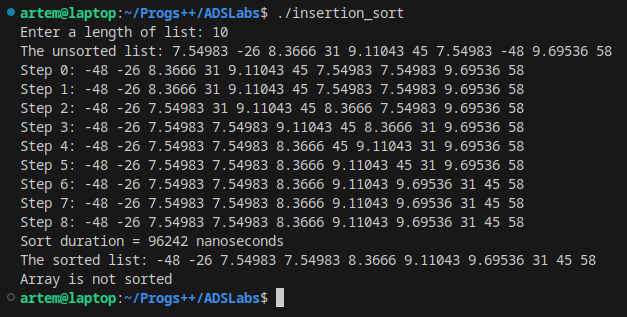
\includegraphics[width=0.90\textwidth]{Screenshot_20231009_222549.png}
    \caption{}
\end{figure}
\subsection*{Висновок} Я навчився змінювати параметри процесів та керувати ними в ОС Linux. Щодо 
завдання 6, можемо бачити що лінукс працює швидше на меншій кількості ядер, він 
працює на 6 ядрах так як віндовс на 12, але при збільшенні ядер до 12 прискорення майже не відбувається.
Можна сказати що лінукс розпаралелює програми більш ефективно.
\end{document}
